\documentclass{emulateapj}
%\documentclass[12pt,preprint]{aastex}

\usepackage[utf8]{inputenc}
\usepackage{graphicx}
\usepackage{float}
\usepackage{amsmath}
\usepackage{epsfig,floatflt}
\usepackage{url}
\setcitestyle{square}

\begin{document}

\title{Project 4}

\author{Stig-Nicolai Foyn}

\email{stignicf@student.matnat.uio.no}

\altaffiltext{1}{Institute of Physics, University of
  Oslo, P.O.\ Box 1029 Blindern, N-0315 Oslo, Norway}

%\date{Received - / Accepted -}

\begin{abstract}
In this study of phase transitions of magnetic systems, we study the Ising model by using Monte Carlo simulation on a binary magnetic spin state lattice.
\end{abstract}

\keywords{Ising model --- computational science --- methods: Monte Carlo, Metropolis Algorithm}

\section{Introduction}
\label{sec:introduction}
This is a study of the Ising model in two dimensions, focusing on utilizing Monte Carlo simulation with the Metropolis algorithm to simulate binary spin states in a lattice with periodic boundary conditions. The different spin-orientations have a set of predictable energies, and the algorithm decides whether a spin should be flipped or not, with a bias towards the equilibrium energy. The Ising model describes phase transitions of magnetic systems without external fields and is characterized by the expression.
%
\begin{equation*}
    E = -J \sum_{kl}^{N} s_{k}s_{l}
\end{equation*}
%
The motivation behind using the Metropolis algorithm is the fact that it only considers the ratio between probabilities. When using the Ising model in two dimentions the partition function has $2^N$ configurations where $N = LxL$. This means that for a $L = 20$ lattice we would have $2^400$ configurations, which is completely unreasonable to calculate, even with a supercomputer. So being able to ignore the partition function means that we can, with relative ease, approximate the characteristics of much larger lattices.

%(Demonstrate usefulness of object-oriented code)

\section{Theory and method}
\label{sec:method}
Finding the analytical results for the $L=2$ spin lattice, will serve as a benefit when benchmarking the precision of the metropolis algorithm. First step is deriving the energy:
%
\begin{equation*}
    Z = \sum_{ \text{All microstates}} e^{-\beta E_{i}} = 2e^{8\beta J} + 12e^{0} + 2e^{-8\beta J}
\end{equation*}
%
Using this identity for $\cosh(x)$:
%
\begin{equation*}
    \cosh(x) = \frac{1}{2} (e^{-x} + e^{x})
\end{equation*}
%
The identity is inserted to the expression found for the partition function:
%
\begin{align*}
    \langle E \rangle &= \frac{\delta ln(Z)}{\delta \beta} = \frac{1}{Z}\frac{\delta Z}{\delta \beta}\\
    &= \frac{1}{Z}\frac{\delta }{\delta \beta} (12 + 4 \cosh(8\beta J))\\
    &= \frac{8 J \sinh({8 \beta J})}{3 +  \cosh({8\beta J})}\\
\end{align*}
%
The heat capacity can now be derived by using the expression below:
%
\begin{align*}
    C_{V} &= \frac{1}{kT^2} \frac{\delta^2 ln(Z)}{\delta \beta^2} = \frac{1}{kT^2} \frac{\delta}{\delta \beta}(\frac{\delta ln(Z)}{\delta \beta})
    = \frac{1}{kT^2} \frac{\delta}{\delta \beta}(\langle E \rangle)\\
    &= \frac{1}{kT^2}\frac{(64 J^2 \cosh({8 \beta J}))(3 + \cosh (8 \beta J)) - 64 J^2 \sinh({8 \beta J}^2)}{(3 + \cosh (8 \beta J))^2}.\\
\end{align*}
%
Magnetization is derived from this expression:
%
\begin{align*}
    \langle |M| \rangle &= \frac{1}{Z} \sum_{i} (M_{i})e^{\beta J E_{i}} \\
    &= \frac{1}{Z}(|4|e^{8\beta J} + 4|2|e^{0} + 0 + 0 + 4|-2|e^{0} + |-4|e^{8\beta J}) \\
    &= \frac{2e^{8\beta J}+4}{3 + \cosh(8\beta J)} \\
\end{align*}
%
And using the expression found for magnetization the susceptibility can be derived as below:
%
\begin{align*}
    \langle M^2 \rangle &= \frac{1}{Z} \sum_{i} (M_{i})e^{\beta J E_{i}} \\
    &= \frac{1}{Z} (2 \times 16e^{8\beta J} + 2 \times 16e^{0}) \\
    \Chi &= \frac{1}{kT}\langle M^2 \rangle = \frac {1}{kT} \frac{8e^{8\beta J} + 8}{3+\cosh(8\beta J)}\\
\end{align*}
%
The numerical results when using the analytical the algorithm
%
\subsection{Ising model}


\subsection{Monte Carlo simulation}

\section{Results}
\label{sec:results}
%
To benchmark the Monte Carlo method analytical values for a $L = 2$ ($2x2$ spin) lattice are used.
%
\begin{deluxetable}{lccc}
%\tablewidth{0pt}
\tablecaption{\label{tab:results1}}
\tablecomments{Table comparing analytical and simulated values found for the L=2 lattice. The expectationvalues from the Monte Carlo model are found using $cycles = 10000$ on one CPU with no cutoff, and $cycles = 1e6$ divided up between 8 CPU threads (effective cycles per thread $cycles = 125000$) with a cutoff at $cycles = 10000$.}
\tablecolumns{3}
\tablehead{Parameter & Analytical & $cycles = 1e4$ & $cycles = 1e6$}
\startdata
$\langle E \rangle$ & -1.99598 & -1.9962 & -1.99609 \\
$\langle |M| \rangle$ & 0.998660  & 0.99865 & 0.998708 \\
$C_{V}$ & 0.03208233 & 0.0303422 & 0.0312116 \\
$\chi$ & 3.993303 & 3.9935 & 3.99351  \\
\enddata
\end{deluxetable}
%
%
\begin{figure}[H]
{{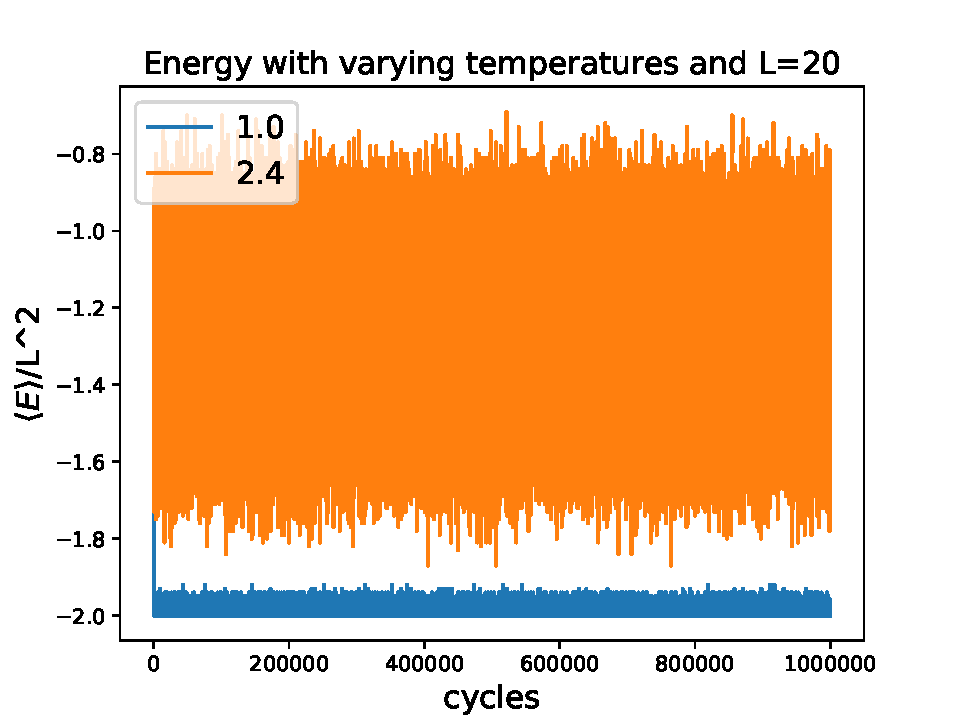
\includegraphics[scale=0.53]{DEL20_MC1M.pdf}}
\subfloat{(a) This plot shows the mean energy for a disordered lattice with temperatures $T=1.0$ and $T=2.4$ for $1e6$ cycles.}
}\qquad
{{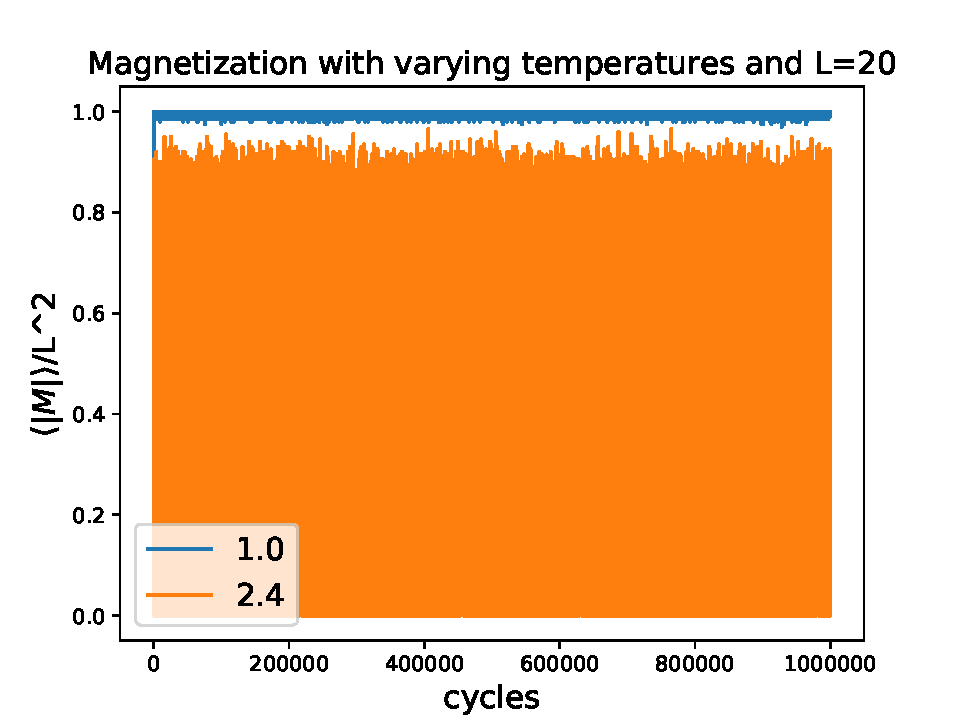
\includegraphics[scale=0.53]{DML20_MC1M.pdf}}
\subfloat{(b) This plot shows the mean magnetization for a disordered lattice with temperatures $T=1.0$ and $T=2.4$ for $1e6$ cycles.}
}\qquad
\caption{Plot for a $L=20$ lattice in ground state, the noise for higher temperatures (and energies) is significant, in addition while not visible in this plot the eqilibration time is at about $500$ cycles.}
\label{fig:Ordered}
\end{figure}
%
%
\begin{figure}[H]
{{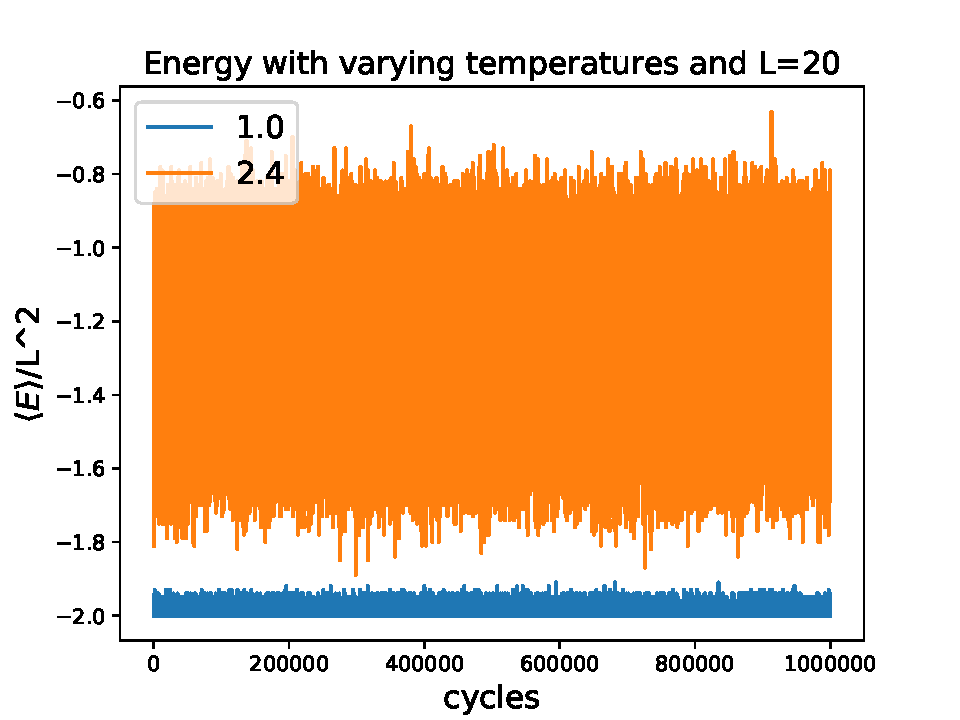
\includegraphics[scale=0.53]{OEL20_MC1M.pdf}}
\subfloat{(a) This plot is the energy for the ordered lattice case, with temperatures $T=1.0$ and $T = 2.4$, using $1e6$ cycles.}
}\qquad
{{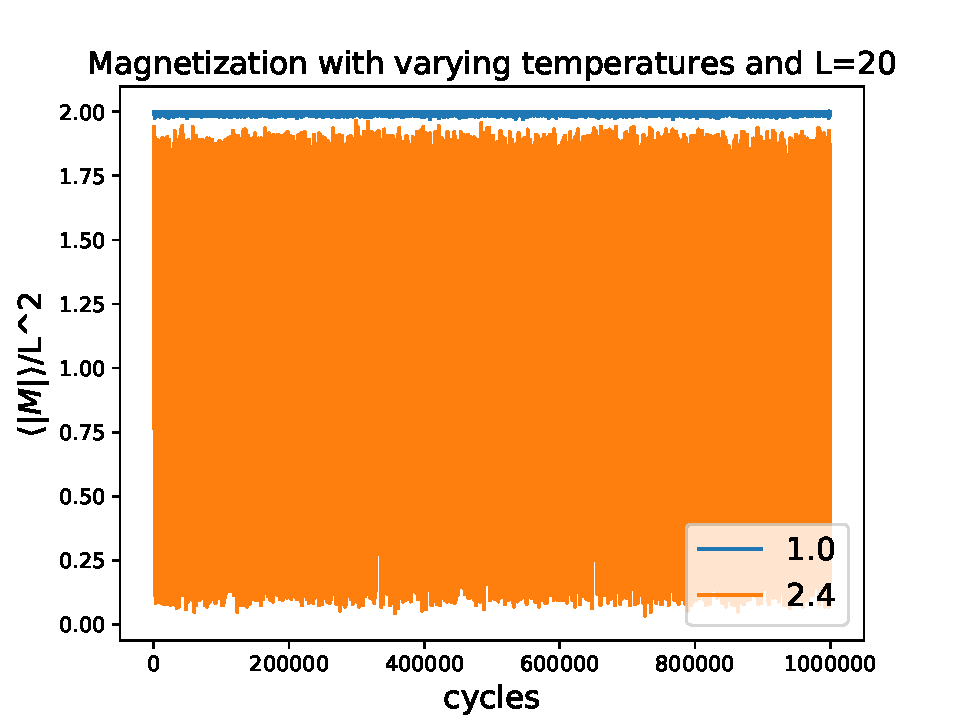
\includegraphics[scale=0.53]{OML20_MC1M.pdf}}
\subfloat{(b) This plot is mean magnetization for the ordered lattice case, for temperatures $T=1.0$ and $T = 2.4$, with $1e6$ cycles.}
}\qquad
\caption{Plot for a $L=20$ lattice in ground state, the most significant difference between this and the disordered lattice case is that the energy and magnetization starts in ground state. This in effect looks similar to having a cutoff value for the disordered state.}
\label{fig:Disordered}
\end{figure}
%
%
\begin{figure}[H]
{{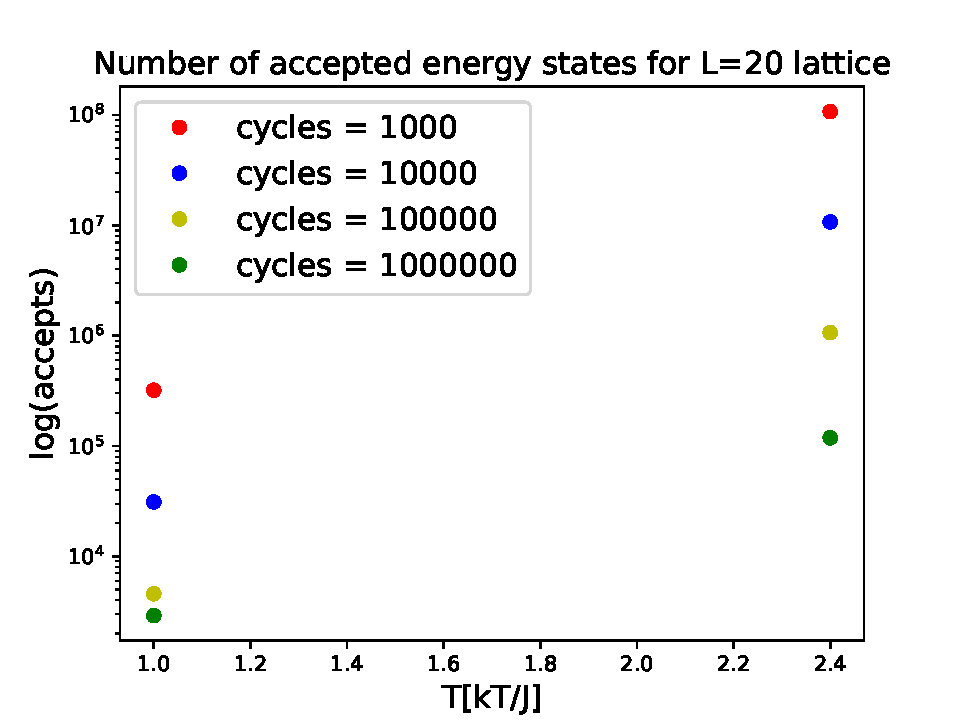
\includegraphics[scale=0.53]{acceptspercyc.pdf}}
\subfloat{(a) Number of accepted states at different amounts of cycles, at temperatures $T = 1.0$ and $T = 2.4$, the amount of cycles does not scale linearly with temperature.}
}\qquad
{{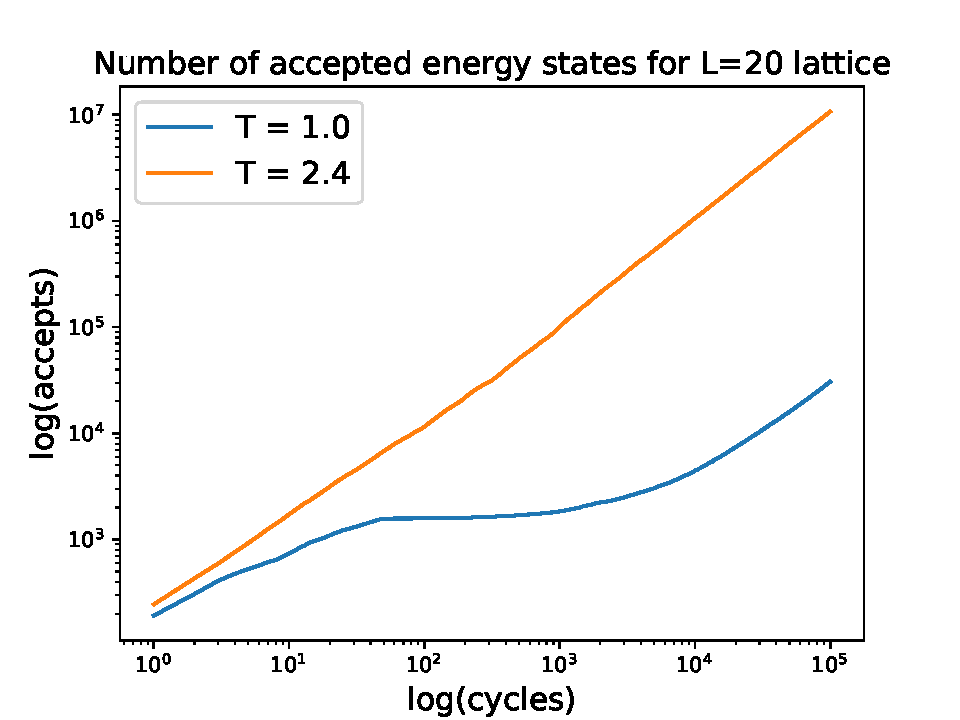
\includegraphics[scale=0.53]{accepts.pdf}}
\subfloat{(b) Number of accepted states as function of the amount of cycles, at temperatures $T = 1.0$ and $T = 2.4$, this to show the temperature dependency on the amount of cycles in a more comprehensive plot.}
}\qquad
\caption{Two different ways to show the amount of accepted energies as function of the amount of cycles and temperature, both run with a $L=20$ lattice.}
\label{fig:accepts}
\end{figure}
%
%
\begin{figure}[H]
{{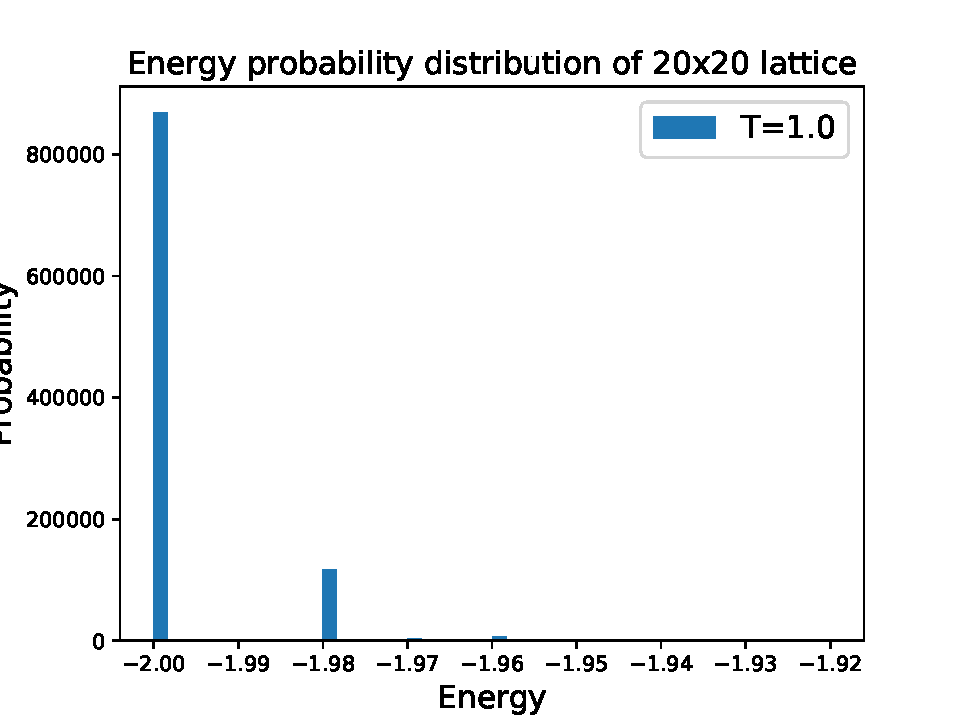
\includegraphics[scale=0.53]{ProbDistribution10_20x20.pdf}}
\subfloat{(a) This plot shows the distribution for temperature $T=1.0$, for low temperatures such as $T=1.0$ the energy distribution favours the ground state energy.}
}\qquad
{{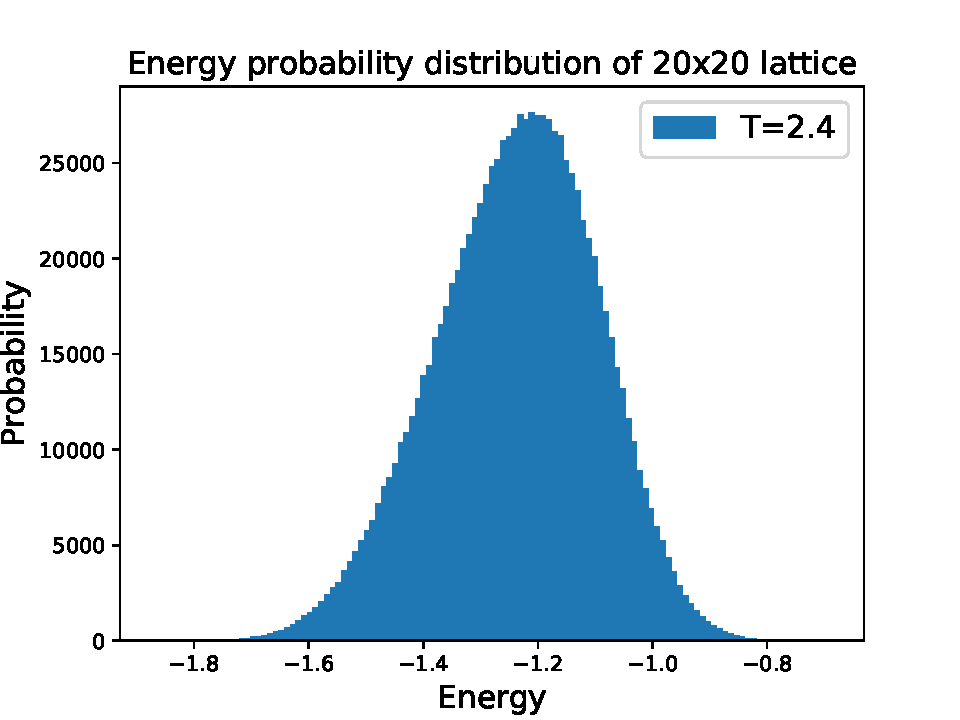
\includegraphics[scale=0.53]{ProbDistribution24_20x20.pdf}}
\subfloat{(b) This plot shows the distribution for temperature $T=2.4$, this looks like a slightly skewed normal probability distribution.}
}\qquad
\caption{This is the energy probability distribution for a $L=20$ lattice with $cycles=1e6$, these distribution histograms are not normalized.}
\label{fig:PD}
\end{figure}
%
The following plots of expectation values were generated on the temperature-interval $T=2.0$ to $T=2.3$ with $dT=0.01$, per temperature the amount of $cycles=1e6$ split between 8 CPU threads with a cutoff at $cycles=10000$.
%
\begin{figure}[H]

\mbox{\epsfig{figure=E_T20-23.pdf,width=\linewidth,clip=}}

\caption{The expectation values for mean energy, the plot seems to reach a turning point right before $T=2.3$.}
\label{fig:Emean}
\end{figure}
%
%
\begin{figure}[H]

\mbox{\epsfig{figure=M_T20-23.pdf,width=\linewidth,clip=}}

\caption{The expectation values for mean magnetic moment, the value decreases until it starts approaching zero where it reaches a turning point, right before $T=2.3$ however there are small spikes of noise cluttering the plot that remain unexplained.}
\label{fig:Mmean}
\end{figure}
%
%
\begin{figure}[H]

\mbox{\epsfig{figure=Cv_T20-23.pdf,width=\linewidth,clip=}}

\caption{The expectation values for heat capacity, it steadily increases until it peaks right before $T=2.3$ however there are large spikes of noise cluttering the plot that remain unexplained.}
\label{fig:HCMean}
\end{figure}
%
%
\begin{figure}[H]

\mbox{\epsfig{figure=Chi_T20-23.pdf,width=\linewidth,clip=}}

\caption{The expectation values for magnetic susceptibility, the plot remains flat for a while before increasing around $T=2.3$ however there are large spikes of noise cluttering the plot that remain unexplained.}
\label{fig:SMean}
\end{figure}
%
The following plots of expectation values were generated on an adjusted temperature-interval from $T=2.2$ to $T=2.4$ with $dT=0.01$, per temperature the amount of $cycles=1e6$ split between 8 CPU threads with a cutoff at $cycles=10000$.
%
\begin{figure}[H]

\mbox{\epsfig{figure=E_T22-24.pdf,width=\linewidth,clip=}}

\caption{The expectation values for mean energy for the adjusted temperature interval, the energy increases steadily until it reaches a turning point right before $T=2.3$.}
\label{fig:Emean2}
\end{figure}
%
%
\begin{figure}[H]

\mbox{\epsfig{figure=M_T22-24.pdf,width=\linewidth,clip=}}

\caption{The expectation values for mean magnetic moment for the adjusted temperature interval, we see a decrease in the magnetic moment and for the larger lattice sizes it approaches zero, which signifies magnetic phase shift.}
\label{fig:Mmean2}
\end{figure}
%
%
\begin{figure}[H]

\mbox{\epsfig{figure=Cv_T22-24.pdf,width=\linewidth,clip=}}

\caption{The expectation values for heat capacity of the lattices, the heat capacities peaks is where our approximation of the critical is found, there are strange artifact found in the graph for some of the lattice sizes ($L=100$ was run multiple times all of them with the same kinds of artifacts at seemingly random places).}
\label{fig:HCMean2}
\end{figure}
%
%
\begin{figure}[H]

\mbox{\epsfig{figure=Chi_T22-24.pdf,width=\linewidth,clip=}}

\caption{The expectation values for magnetic susceptibility, the peak of the plot is where the critical temperature $T_C$ is found, however there seems to be a lot of noise in some of the values, especially considering the spike at $L=100$.}
\label{fig:SMean2}
\end{figure}
%
%
\begin{figure}[H]

\mbox{\epsfig{figure=Tc_LinFit.pdf,width=\linewidth,clip=}}

\caption{Lienar regression of the max values of the magnetic susceptibilities (where we approximate $T_C$ to be) for different matrix dimensionality $L^2$, the value of $T_C$ approximated in this regression is $2.263187$, and the equation of the curve is $y = 1.440913T + T_C$.}
\label{fig:LinearFitting}
\end{figure}
%
The program Critical.py renders a plot of the linear fitting of our expectation values and prints the value where this plot would cross the y-axis. This is where the critical temperature would have been if we let $L \rightarrow \infty$ which is also the expected exact value (found by Lars Onsager) $kT_{c}/J = 2/ln(1+\sqrt{2}) \approx 2.269$ for $\nu = 1$ (from \cite{bib:project4}).

\section{Discussion}
\label{sec:discussion}
We consider the accuracy of the implemented metropolis algorithm, by comparing the approximated values to the analytical ones. As seen in table.\ref{tab:results1} the accuracy of most of the expectation values are relatively close to the analytical value for $cycles = 1e4$, and even closer still for $cycles = 1e6$, which is why this is the amount of cycles used for later analysis.

\section{Conclusions}
\label{sec:conclusions}



\begin{acknowledgements}

\end{acknowledgements}

\begin{thebibliography}{}
\bibitem{bib:project4} Hjorth-Jensen, Morten, 2018, \textit{Project 4} \url{http://compphysics.github.io/ComputationalPhysics/doc/
Projects/2018/Project4/pdf/Project4.pdf} (24.10.18)

\bibitem{}
\end{thebibliography}


\end{document}
